\documentclass[dvips,xcolor=pst,14pt]{beamer}
%\documentclass[dvips,handout,xcolor=pst]{beamer}
%\documentclass[letterpaper]{article}
%\usepackage{beamerarticle}
%\newcommand{\newblock}{} % a hack for bibtex.
\usepackage{color}
\usepackage{pstricks}
%\usepackage{hyperref}
%\usepackage[authoryear]{natbib}
\usepackage{graphicx}
\usepackage{multimedia}
\usepackage{pgfpages}
\usepackage{arydshln}
\usepackage{commath}
\usepackage{vector}
%\usepackage{cancel}
\usepackage{ulem}
\usepackage{listings}
%\usepackage{times}

\graphicspath{{pyhpc_eps/}}

\newcommand{\defeq}{\ensuremath{\buildrel {\text{def}}\over{=}}} 

\usetheme{CambridgeUS}
%\usefonttheme[stillsansseriftext]{serif}
\usefonttheme[onlymath]{serif}

%\setbeameroption{show notes}
%\setbeameroption{show only notes}
%\pgfpagesuselayout{2 on 1}[letterpaper,border shrink=0.2in]

\lstset{basicstyle=\footnotesize\ttfamily,%
keywordstyle=\color{blue},%
stringstyle=\color{magenta},%
commentstyle=\color{red},%
breaklines=true}
%\lstset{framextopmargin=50pt,frame=bottomline}

\title[SciPy]{Robust Platform for Scientific Computing: Python}
%
\author[\href{http://solvcon.net/yyc/}{Yung-Yu Chen}]%
{\href{http://solvcon.net/yyc/}{Yung-Yu Chen} \\ {\scriptsize
\url{yyc@solvcon.net}}}
%
\institute[PyHUG]{Python Hsinchu User Group}
%
\date[2013/9/24]{September 24, 2013}

\begin{document}

\begin{frame}
\titlepage
\end{frame}

\section*{
%%%
Outline
%%%
}

\begin{frame}{
%
Topics
%
}
\tableofcontents
\end{frame}

\section{
%%%
The Need for Scientific Computing
%%%
}

\subsection{
%%
The State of the Art
%%
}

\begin{frame}{
%
Supercomputing
%
}
\begin{columns}
  \begin{column}{0.25\textwidth}
    \centering
    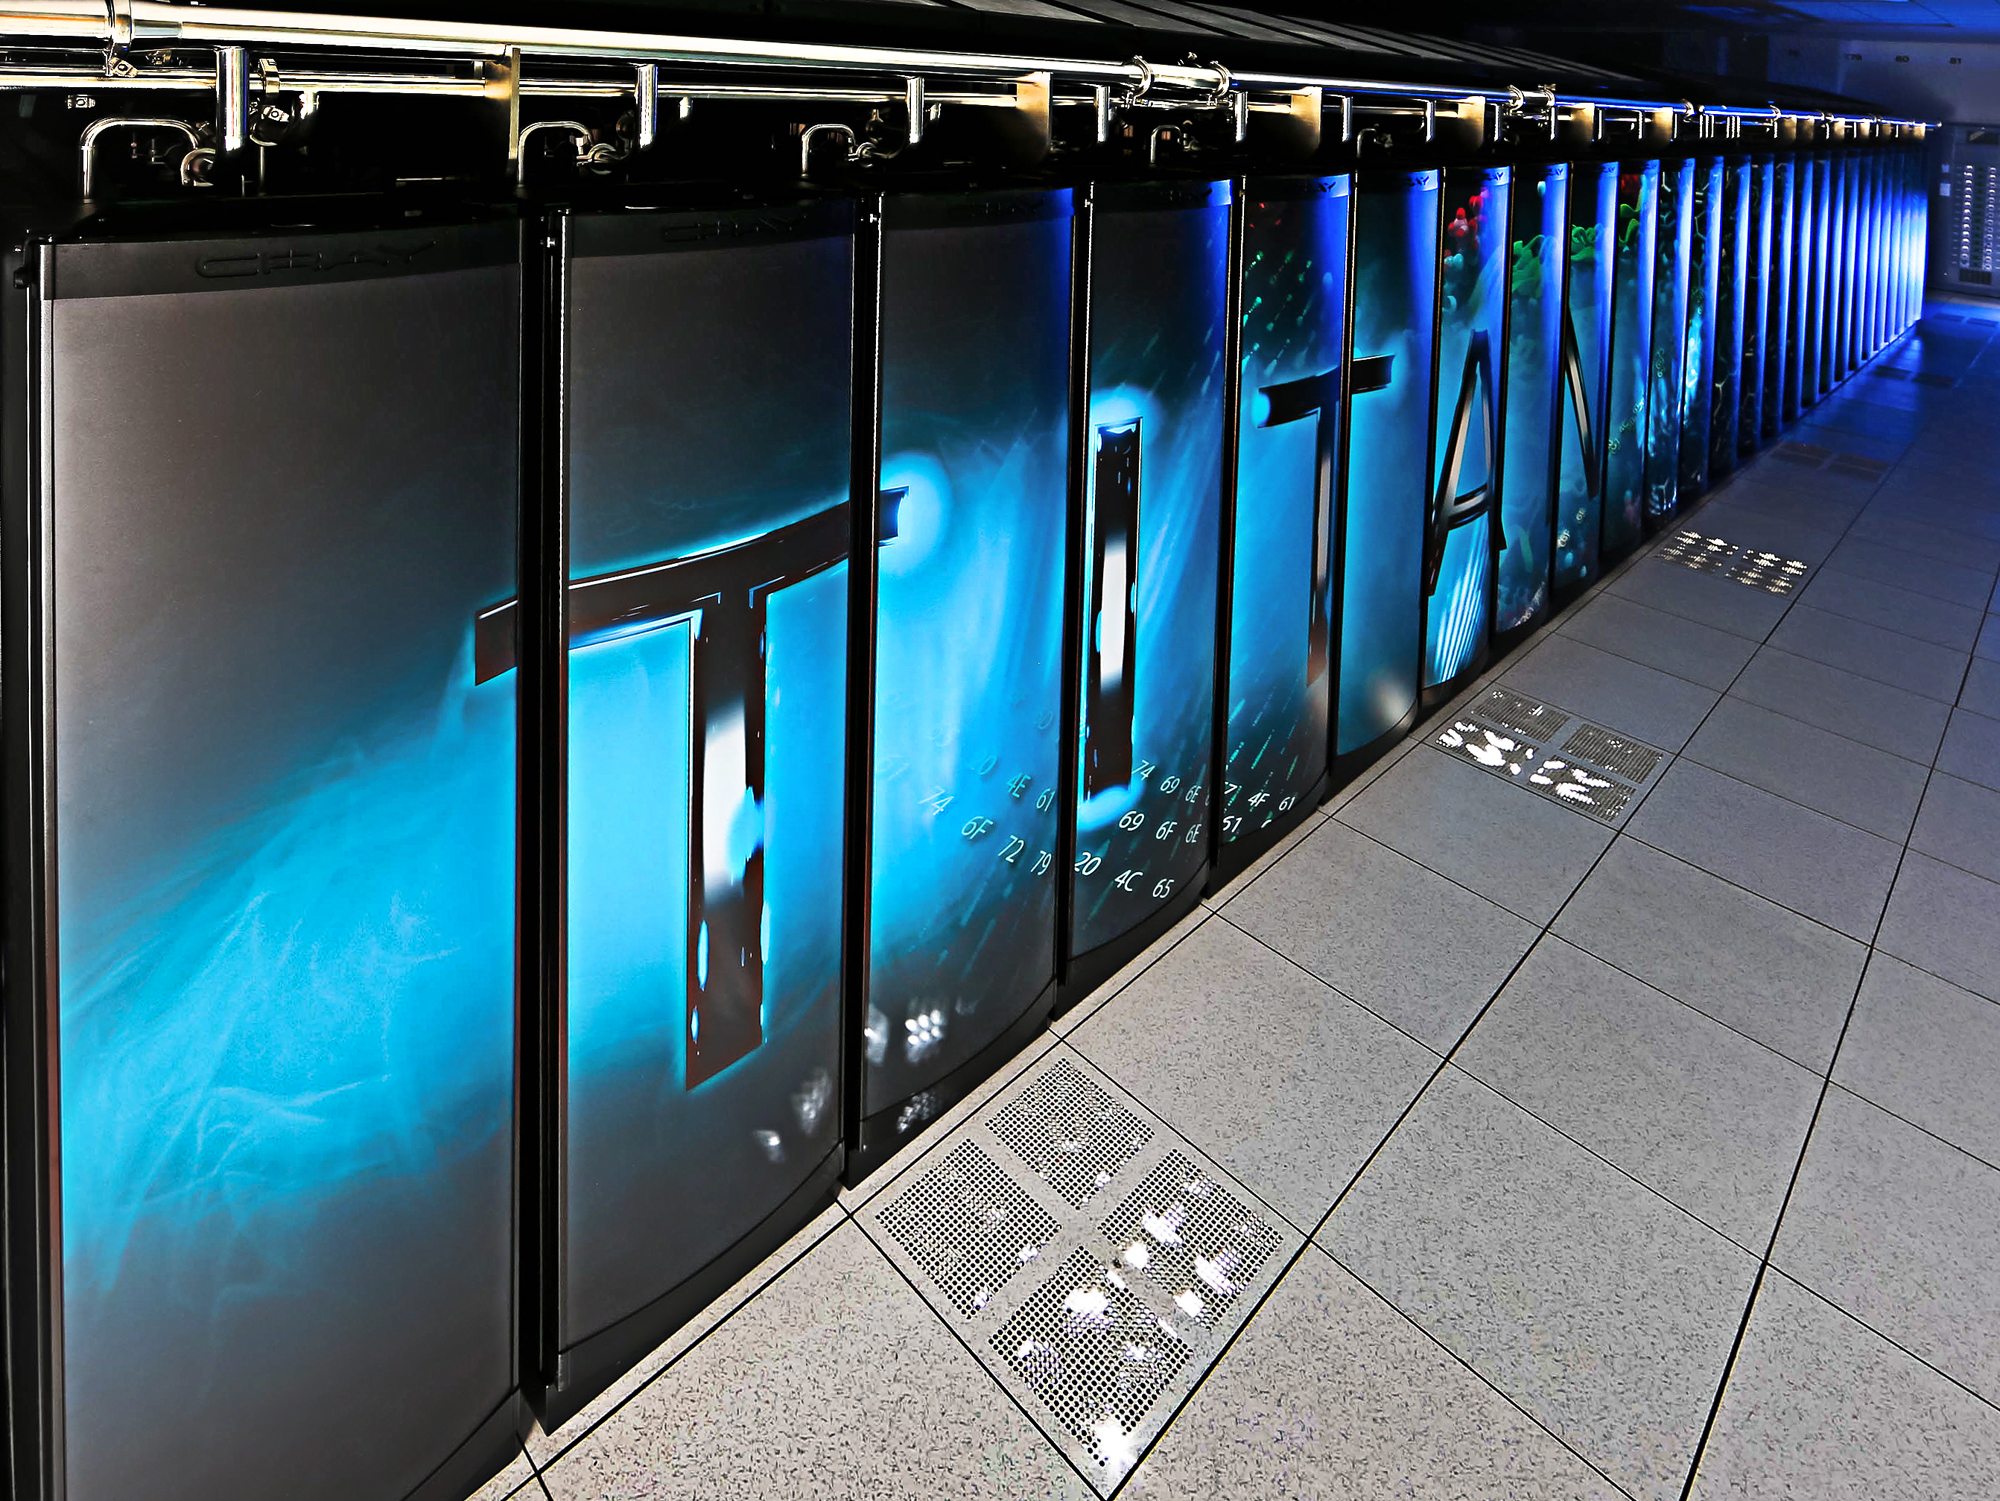
\includegraphics[width=\textwidth]{titan3.eps}
  \end{column}
  \begin{column}{0.75\textwidth}
    \begin{itemize}
      \item Specialized hardware for specific applications.
      \item \alert{Speed} is the number 1 objective.
    \end{itemize}
  \end{column}
\end{columns}
\begin{itemize}
\item Top 500 list ({\small\url{http://top500.org/lists/2013/06/}}):
\begin{enumerate}
  \item Tianhe-2: 3.12M cores, 33.86 Pflops (Peta floating-point operations per
  second).  Equips Xeon E5-2692 and Xeon-Phi 31S1P.
  \item Titan (Cray XK7): 0.56M cores, 17.59 Pflops.  Equips Opteron 6274 and
  NVIDIA K20x.
  \item Sequoia (IBM BlueGene/Q): 1.57M cores, 17.17 Pflops.  Equips Power PQC 16C.
\end{enumerate}
\end{itemize}
\end{frame}

\begin{frame}{
%
Cloud Computing
%
}
\begin{columns}
  \begin{column}{0.35\textwidth}
    \centering
    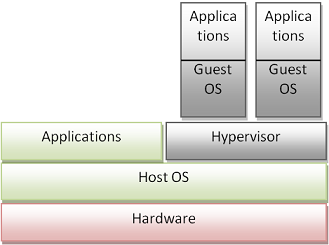
\includegraphics[width=\textwidth]{virtualization.eps}
  \end{column}
  \begin{column}{0.65\textwidth}
    \begin{itemize}
    \item Provide \alert{elastic} computing power through virtualization
    technology.
    \begin{itemize}
      \item Programs are run not on real hardware, but the virtualized systems.
      \item Users can dynamically allocate resources including computing nodes and
      cores, memory, storage, etc.
    \end{itemize}
    \end{itemize}
  \end{column}
\end{columns}
\begin{itemize}
  \item Pay-as-you-go allows everyone to solve significantly large problems.
\end{itemize}
\end{frame}

\begin{frame}{
%
But This Is Really We Are Using
%
}
\begin{center}
  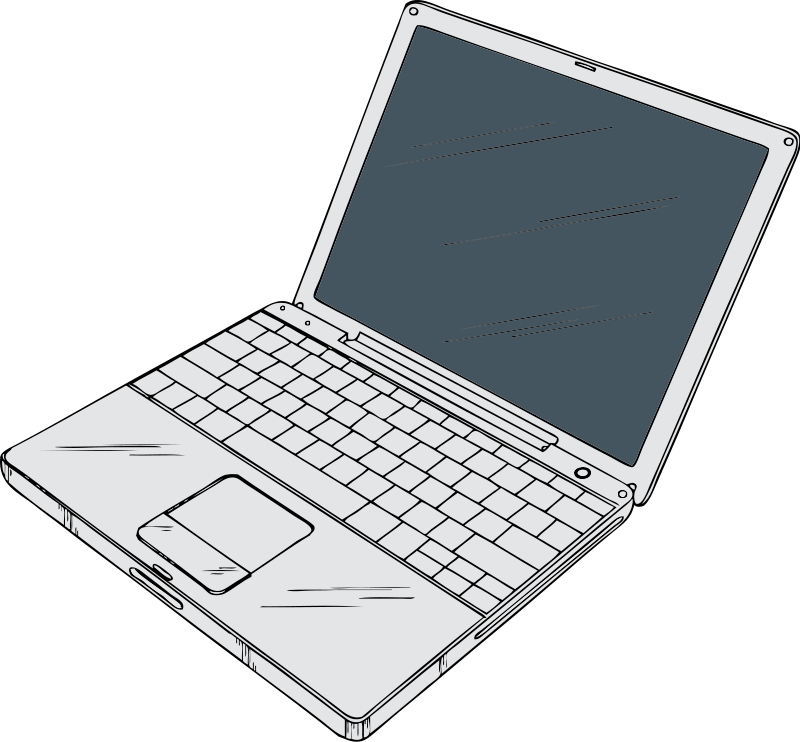
\includegraphics[height=0.6\textheight]{laptop.eps}
\end{center}
\end{frame}

\begin{frame}{
%
Programming Platform Matters
%
}
\begin{itemize}
  \item You need a programming language, or several programming languages, to
  process, simulate, analyze, and exhibit the data of your problems.
  \begin{itemize}
    \item It doesn't matter what supercomputers you are using.
    \item It doesn't matter what cloud services you are using.
    \item It doesn't matter if you are running the code on your laptop.
  \end{itemize}
  \item You need to be proficient at a powerful programming language.
  \item And Python is that language.
\end{itemize}
\end{frame}

\subsection{
%%
Python Supports Scientific Computing
%%
}

\begin{frame}[fragile]{
%
What Python Can Do?
%
}
\begin{itemize}
  \item An everyday tool:
  {\small \verb+python -c 'import math; print math.factorial(10)'+}.
  \item An established ecosystem for reproducible analysis.
  \begin{itemize}
    \item A rich collection of scientific tools: NumPy, SciPy, Matplotlib,
    Pandas, iPython, etc.
  \end{itemize}
  \item A popular platform for web programming.
  \begin{itemize}
    \item Even include a web server: {\small \verb+python -m SimpleHTTPServer+}.
  \end{itemize}
  \item A platform that allows you to do anything.
  \begin{itemize}
    \item The Python Package Index (\url{https://pypi.python.org/pypi}) now has
    34,924 packages.
  \end{itemize}
\end{itemize}
\end{frame}

\begin{frame}{
%
A Rich Interactive Environment
%
}
\begin{center}
  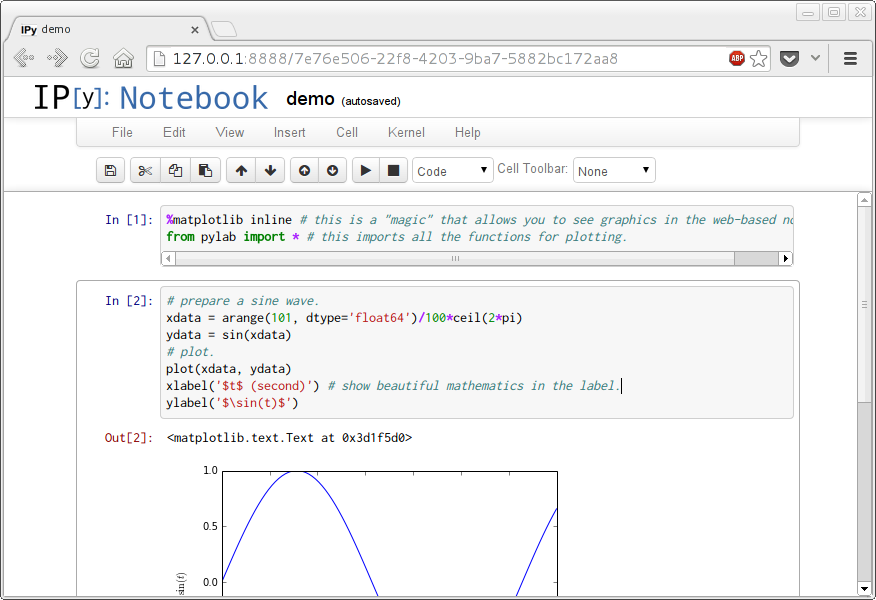
\includegraphics[width=0.85\textwidth]{ipython_nb.eps}
\end{center}
\end{frame}

\section{
%%%
The Python Ecosystem
%%%
}

\subsection{
%%
Getting Start
%%
}

\begin{frame}{
%
Before Started
%
}
\begin{itemize}
  \item The Python official site contains comprehensive information:
  \begin{itemize}
    \item Table of contents of the documentation:
    \url{http://docs.python.org/2/}.
    \item The best reference to the standard library:
    \url{http://docs.python.org/2/library/index.html}.
    \item Read \textit{The Python Tutorial}
    (\url{http://docs.python.org/2/tutorial/index.html}).
  \end{itemize}
  \item Start with Python \alert{2}.
  \item A good self-training material is \textit{Learn Python the Hard Way}
  (\url{http://learnpythonthehardway.org/book/}).
\end{itemize}
\end{frame}

\begin{frame}{
%
Installation
%
}
\begin{itemize}
  \item Use Anaconda.
  \begin{itemize}
    \item \url{https://store.continuum.io/cshop/anaconda/}.
    \item It provides everything at once and can be easily updated.
  \end{itemize}
  \item NOT recommended for scientific users:
  \begin{itemize}
    \item Download from Python website.
    \item Use your OS's package managers (apt-get, yum, ports, etc.)
  \end{itemize}
  \item Why not?
  \begin{itemize}
    \item They require expertise in Python and take long time.
    \item They contains outdated packages.
  \end{itemize}
\end{itemize}
\begin{flushleft}
  \scriptsize *This suggestion is specific to scientific users.
\end{flushleft}
\end{frame}

\begin{frame}{
%
Two Types of Programming
%
}
\begin{itemize}
  \item Compiled vs interactive.
  \begin{itemize}
    \item Low-level platform is built upon pre-compiled executables, like the
    Python runtime and the underneath libraries.
    \item In a high-level interactive environment, we can type just several
    commands or press buttons to do complex computing.
  \end{itemize}
  \item Python glues the low-level parts together, and expose them to the
  high-level.
  \item To configure and build the low-level platform needs a lot of efforts.
  \begin{itemize}
    \item Products like Anaconda do that for us.
  \end{itemize}
\end{itemize}
\end{frame}

\subsection{
%%
Scientific Python Toolkits
%%
}

\begin{frame}{
%
Categories of Scientific Python Tools
%
}
\begin{itemize}
  \item Programming.
  \begin{itemize}
    \item \alert{NumPy}, \alert{Cython}, \alert{iPython}.
  \end{itemize}
  \item Algorithms.
  \begin{itemize}
    \item \alert{SciPy}, SciKits.
  \end{itemize}
  \item Visualization.
  \begin{itemize}
    \item \alert{Matplotlib}, VTK.
  \end{itemize}
  \item Applications.
  \begin{itemize}
    \item Pandas, NLTK, networkx, PyMOL, Pyomo, yt, ..., etc.
  \end{itemize}
\end{itemize}
\end{frame}

\begin{frame}[fragile]{
%
NumPy
%
}
\begin{itemize}
  \item NumPy ({\small \url{http://numpy.scipy.org/}}) provides basic
  multi-dimensional array support.
  \item Array-oriented programming is the foundation to scientific computing.
  \item It provides basic facilities such as linear algebra and Fourier
  transform.
\end{itemize}
Let's see the demo.
\end{frame}

\begin{frame}[fragile]{
%
Cython
%
}
\begin{itemize}
  \item Cython ({\small \url{http://cython.org/}}) is a superset of the Python
  programming language.
  \item It speeds up Python code to be comparable of C.
  \item It provides interfaces for Python to use low-level C code or libraries.
\end{itemize}
\end{frame}

\begin{frame}[fragile]{
%
Cython Benchmark
%
}
\begin{lstlisting}[basicstyle=\tiny\ttfamily,language=Python,escapechar=!]
import numpy as np
!\colorbox{red}{cimport numpy as cnp}!
def action():
    !\colorbox{red}{cdef cnp.ndarray[cnp.double\_t, ndim=2]}! arr0 = np.empty([1000,1000], dtype='float64')
    arr0.fill(0)
    !\colorbox{red}{cdef cnp.ndarray[cnp.double\_t, ndim=2]}! arr1 = np.empty([1000,1000], dtype='float64')
    arr1.fill(1)
    !\colorbox{red}{cdef int}! it = 1
    !\colorbox{red}{cdef int}! jt
    while it < 999:
        jt = 1
        while jt < 999:
            arr0[it, jt] += arr1[it-1, jt-1]
            arr0[it, jt] += arr1[it-1, jt  ]
            arr0[it, jt] += arr1[it-1, jt+1]
            arr0[it, jt] += arr1[it  , jt+1]
            arr0[it, jt] += arr1[it+1, jt+1]
            arr0[it, jt] += arr1[it+1, jt  ]
            arr0[it, jt] += arr1[it+1, jt-1]
            arr0[it, jt] += arr1[it  , jt-1]
            jt += 1
        it += 1
    assert 7968032 == arr0.sum()
\end{lstlisting}
\small Cython is \alert{41} times faster than normal Python.
\end{frame}

\begin{frame}[fragile]{
%
iPython Notebook
%
}
\begin{itemize}
  \item iPython stands for interactive Python.
  \item It provides plain-text, GUI, and web interface.
  \item iPython notebook is its web interface.
  \begin{itemize}
    \item Use {\small \verb+ipython notebook+} to launch.
    \item Useful for research notes, experimenting, and education.
    \item Mathematical expressions are the first-class citizen.
    \item You can store and share any ipython notebook, even online:
    \url{http://nbviewer.ipython.org/}.
  \end{itemize}
\end{itemize}
Let's see more demo of it.
\end{frame}

\begin{frame}[fragile]{
%
SciPy Library
%
}
\begin{itemize}
\item The term SciPy has many meanings:
  \begin{itemize}
    \item The SciPy library ({\small
    \url{http://docs.scipy.org/doc/scipy/reference/}}); what I want to talk
    about here.
    \item The SciPy ecosystem ({\small \url{http://www.scipy.org/}});
    everything about Python for sciences.
    \item The SciPy conference ({\small \url{http://conference.scipy.org/}});
    in North America, Europe, and India.
    \item The SciPy community; those who use Python for scientific research.
  \end{itemize}
\end{itemize}
Let's see how it works in an ipython notebook.
\end{frame}

\section{
%%%
HPC Code Development for Research
%%%
}

\begin{frame}{
%
It's about SOLVCON
%
}
 A solver constructor.
\begin{itemize}
  \item Perform first-principle simulations for physical processes governed
  by conservation laws.
  \begin{itemize}
    \item Usually formulated as hyperbolic partial differential equations
    (PDEs).
  \end{itemize}
  \item Written in \alert{Python} and with the performance hot-spot
  accelerated by C (or CUDA).
  \item Address \alert{high-performance computing (HPC)} by mesh-based,
  array-oriented programming.
\end{itemize}
See \url{http://solvcon.net/} for detail.
\end{frame}

\subsection{
%%
First-Principle Simulations and Conservation Laws
%%
}

\begin{frame}{
%
Conservation Laws Govern The World
%
}
\begin{center}
  Fluid mechanics, solid mechanics, electromagnetism, etc.
  \begin{minipage}{0.32\textwidth} \centering
  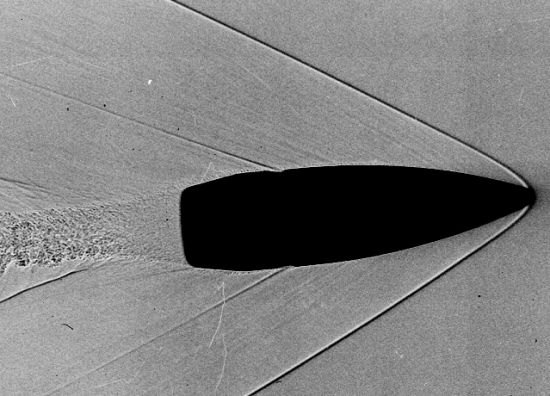
\includegraphics[width=\textwidth]{supersonic_bullet.eps} \\
  \small Supersonic flow.
  \end{minipage}
  \hskip 1em
  \begin{minipage}{0.32\textwidth} \centering
  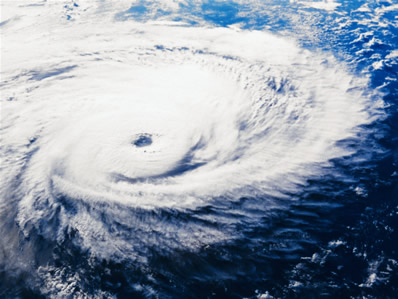
\includegraphics[width=\textwidth]{climate.eps} \\
  \small Atmospheric flow.
  \end{minipage}
  \hskip 1em
  \begin{minipage}{0.25\textwidth} \centering
  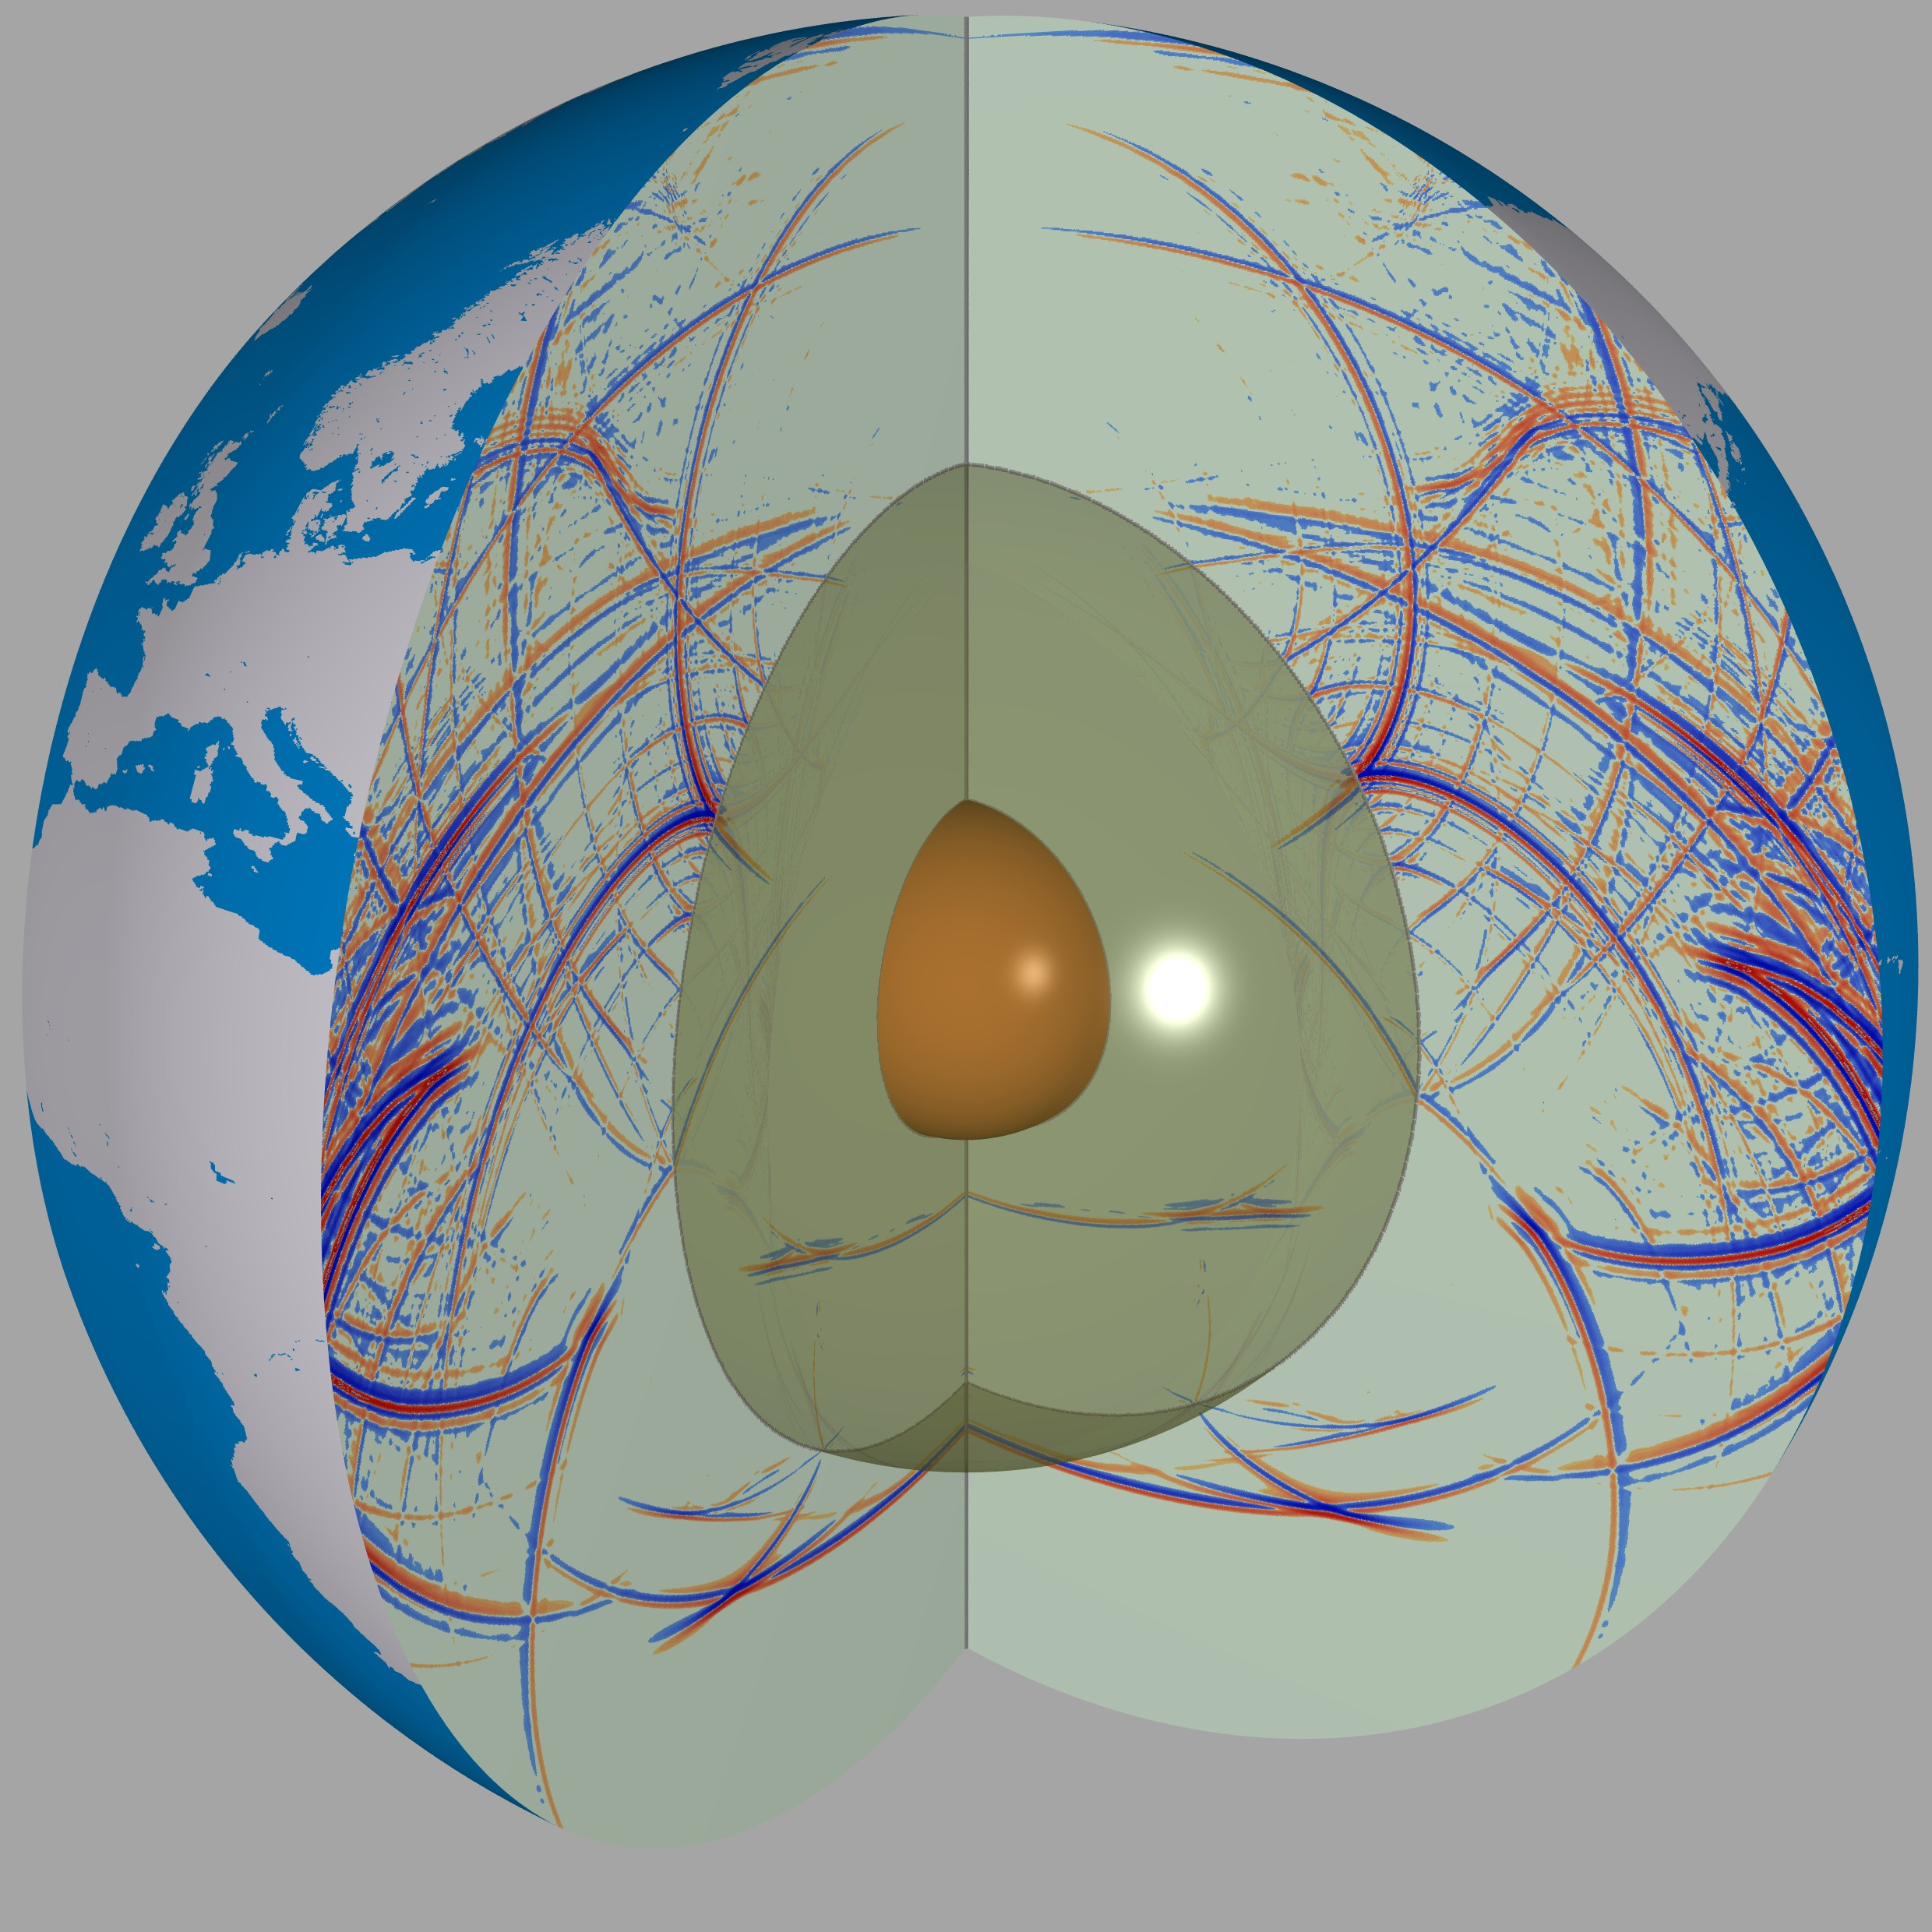
\includegraphics[width=\textwidth]{seismic_wave.eps} \\
  \small Seismic waves.
  \end{minipage}
\end{center}
\begin{center}
  \begin{minipage}{0.4\textwidth} \centering
  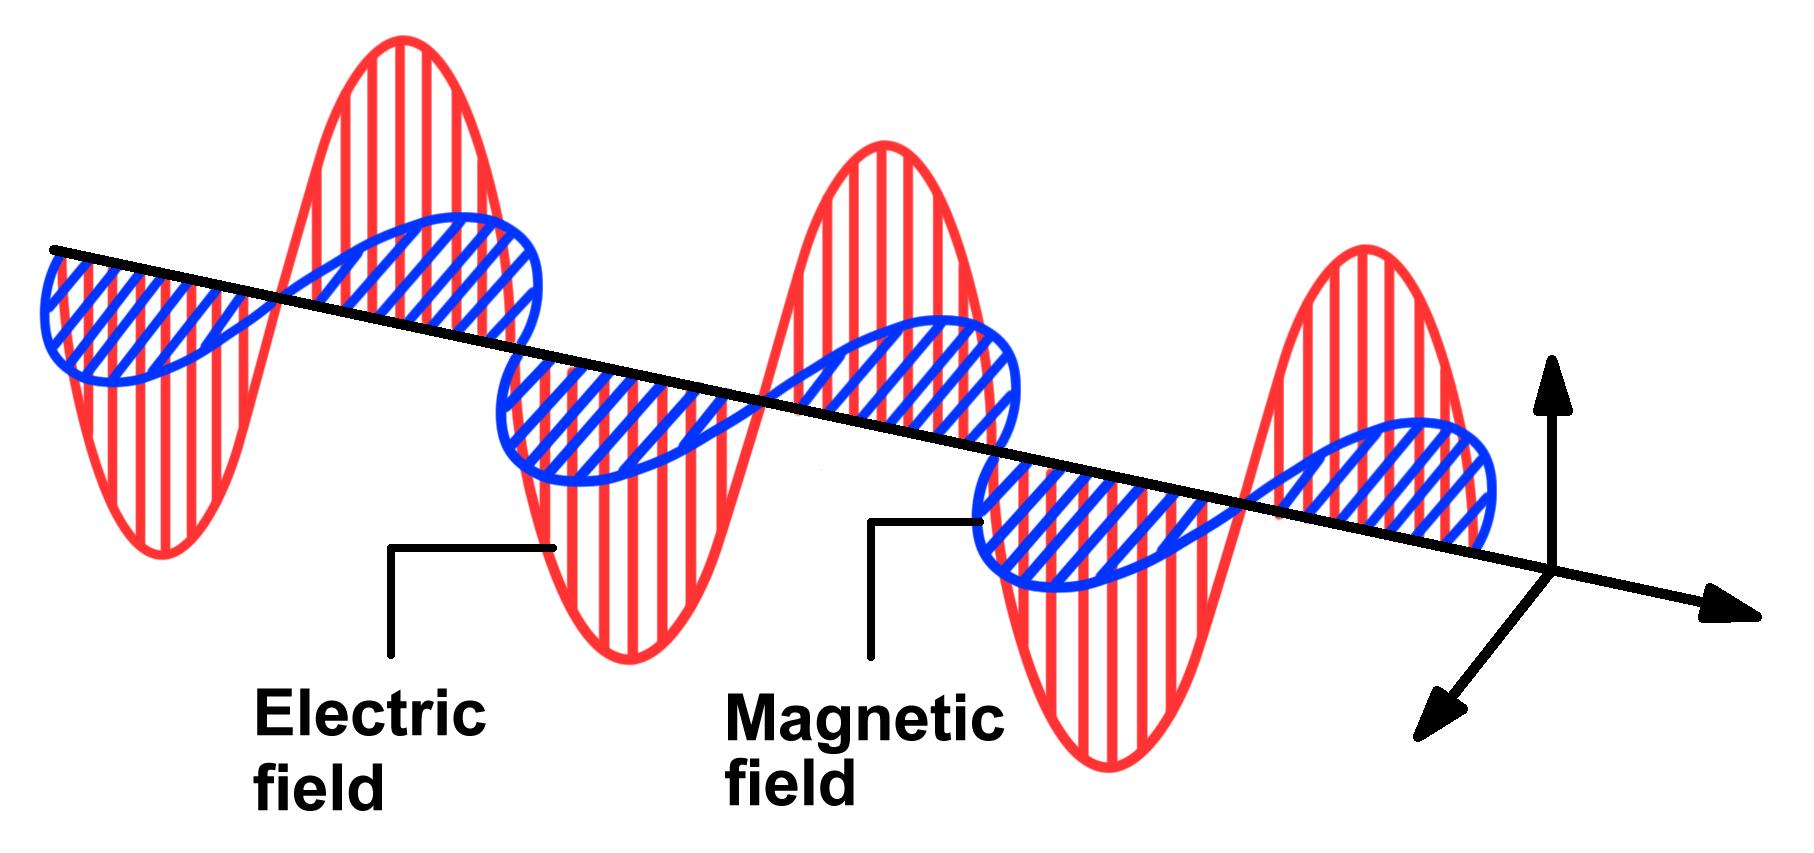
\includegraphics[width=\textwidth]{emwave.eps} \\
  \small Electromagnetic waves.
  \end{minipage}
\end{center}
\end{frame}

\begin{frame}{
%
First-Order Hyperbolic PDEs
%
}
\begin{itemize}
  \item The fore-mentioned problems share a common trait: Demanding
  time-accurate solutions of conservation laws.
  \item So this is what I want to solve:
  {\footnotesize \begin{align}
   &\frac{\partial u_m}{\partial t}
      + \sum_{\mu=1}^3\frac{\partial f^{(\mu)}_m(\bvec{u})}{\partial x_{\mu}}
      = s_m(\bvec{u}) \notag \\
    \Rightarrow \quad &\boxed{\begin{gathered}
      \oint_{S(V)}\bvec{h}_m(\bvec{u})\cdot d\bvec{a}
      = \int_{V}s_m(\bvec{u})dv
    \end{gathered}} \label{e:conserv} \\
   &m = 1, \ldots, M. \notag
  \end{align}}
\end{itemize}
\end{frame}

\begin{frame}{
%
Challenges in Programming
%
}
Coding for first-principle simulators is difficult.  Why?
\begin{enumerate}
  \item Recall the math:
  {\footnotesize \begin{align}
   \frac{\partial u_m}{\partial t}
      + \sum_{\mu=1}^3\frac{\partial f^{(\mu)}_m(\bvec{u})}{\partial x_{\mu}}
      = s_m(\bvec{u}) \tag{\ref{e:conserv}}
  \end{align}}
  \item Various approaches to meshing and the associated data structures.
  \item Parallel programming for HPC.
  \item Data management and result analysis.
\end{enumerate}
\end{frame}

\begin{frame}{
%
The CESE Method
%
}
\begin{itemize}
  \item The space-time Conservation Element and Solution Element
  (\href{http://www.grc.nasa.gov/WWW/microbus/}{CESE}) method, developed by
  Chang at NASA Glenn.
  \begin{itemize}
    \item Directly solves generic hyperbolic PDEs (Eq.~\eqref{e:conserv}).
  \end{itemize}
  \item Enable pluggable multi-physics in SOLVCON.
  \begin{itemize}
    \item Compressible flows: $\bvec{u} = (\rho, \rho v_1, \rho v_2, \rho v_3,
    \rho e)^t$.
    \item Stress waves in solids: $\bvec{u} = (v_1, v_2, v_3, \sigma_{11},
    \sigma_{22}, \sigma_{33}, \sigma_{23}, \sigma_{13}, \sigma_{12})^t$.
    \item Electromagnetic waves: $\bvec{u} = (E_1, E_2, E_3, B_1, B_2, B_3)^t$.
    \item Acoustics, shallow-water, viscoelasticity, etc.
  \end{itemize}
\end{itemize}

\begin{flushright}\footnotesize
\href{http://dx.doi.org/10.1006/jcph.1995.1137}{Chang (1995) Journal of
Computational Physics 119(2):295--324} \\
\href{http://solvcon.net/yyc/publications.html}{Chen (2011), Ph.D. Dissertation}
\end{flushright}

\end{frame}

\subsection{
%%
SOLVCON
%%
}

\begin{frame}{
%
What Is SOLVCON
%
}
\begin{itemize}
  \item A Python-based software framework for constructing time-accurate
  solvers of conservation laws for any physical processes.
  \item SOLVCON uses the CESE method.
  \begin{itemize}
    \item Unstructured meshes of mixed elements are used in two- or
    three-dimensional space.
    \item Message-passing is built into the framework for parallel computing.
  \end{itemize}
\end{itemize}
\end{frame}

\begin{frame}{
%
Application: Stress Wave in Solids
%
}
\begin{itemize}
  \item Beryl: Anisotropic crystal of hexagonal symmetry.
\end{itemize}
\begin{center}
  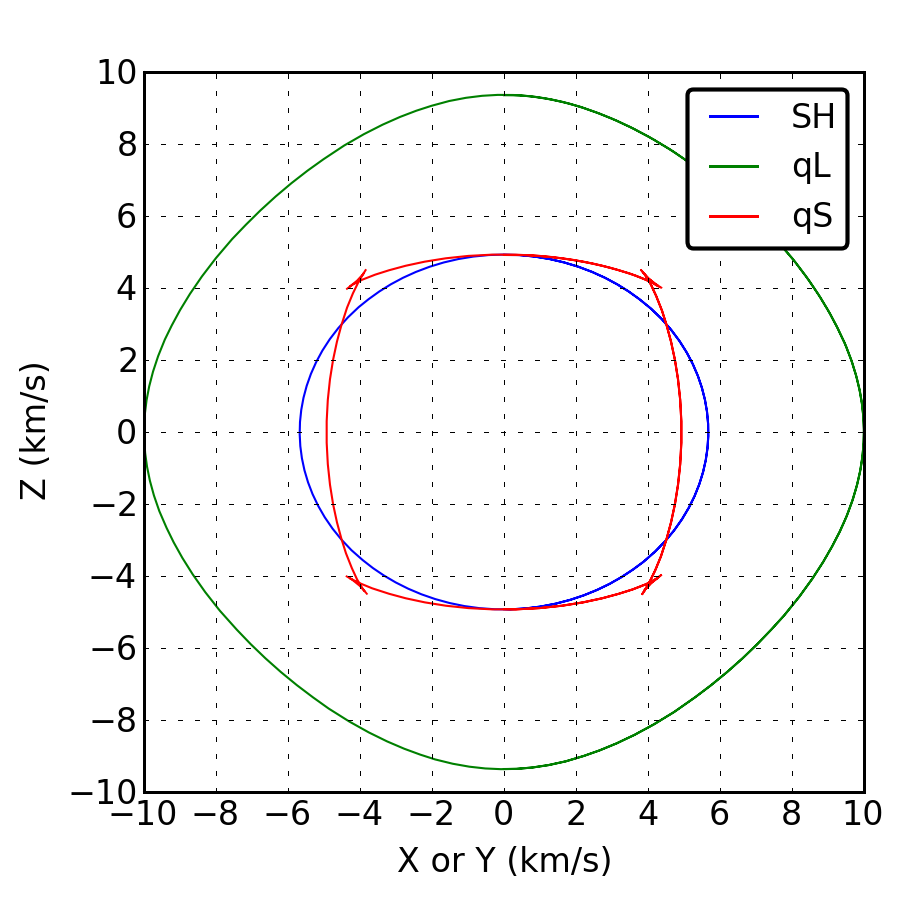
\includegraphics[width=0.4\textwidth]{Beryl.eps}
  \hskip 0.5em
  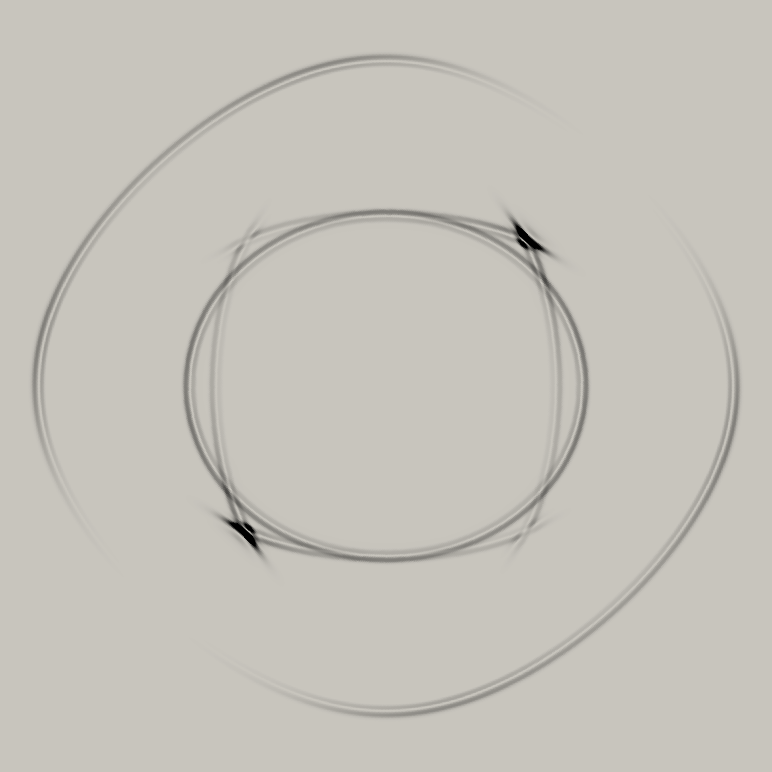
\includegraphics[width=0.4\textwidth]{Beryl_sim_white.eps}
  \\
  \parbox[t]{0.4\textwidth}{\footnotesize \centering Exact solution of group velocity}
  \hskip 1em
  \parbox[t]{0.4\textwidth}{\footnotesize \centering Simulated result}
\end{center}

\parbox{\textwidth}{\raggedleft \footnotesize
\href{http://dx.doi.org/10.1115/1.4002170}{Yang et al. (2011) J.  Vib. Acoust.
133(2): 021001}}
\end{frame}

\begin{frame}{
%
Application: Supersonic Flows
%
}
\begin{columns}[c]
\begin{column}{.6\textwidth}
\begin{center}
  \begin{minipage}[c]{\textwidth} \centering
    \parbox{0.3\textwidth}{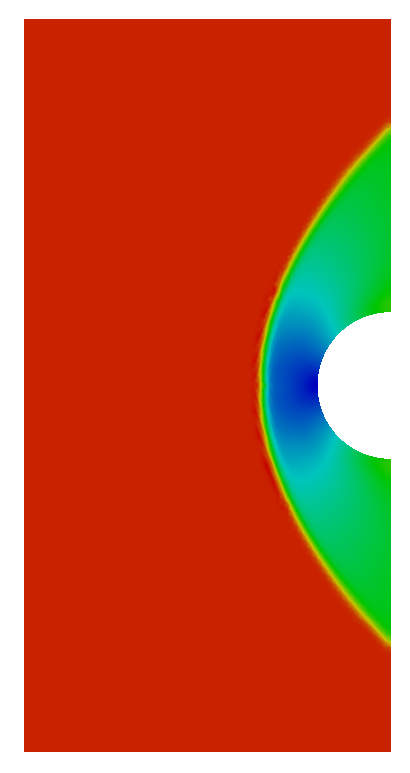
\includegraphics[width=0.3\textwidth]{foc_m3.eps}}
    \hfill
    \parbox{0.65\textwidth}{%
    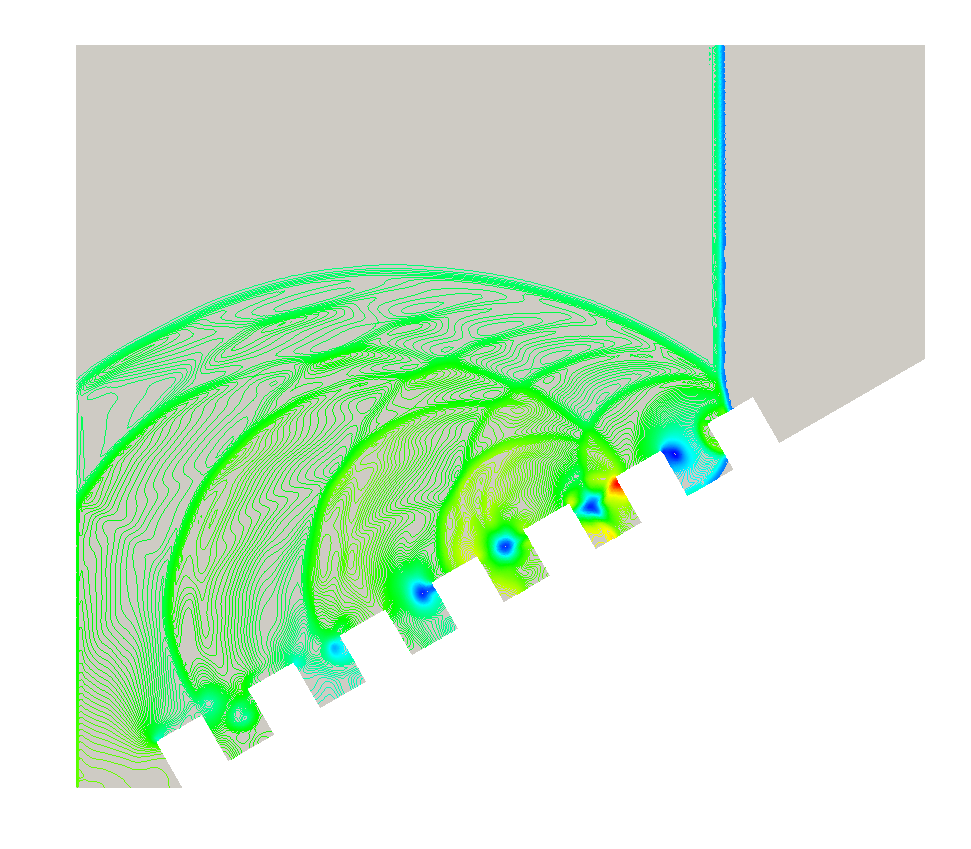
\includegraphics[width=0.65\textwidth]{dust_layer.eps}}
  \end{minipage} \\
  \begin{minipage}[c]{\textwidth} \centering
    \parbox{\textwidth}{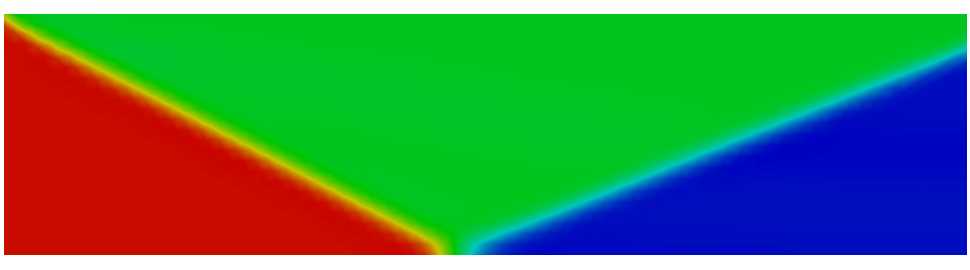
\includegraphics[width=\textwidth]{refl_m3.eps}}
  \end{minipage}
\end{center}\end{column}
\begin{column}{.4\textwidth}
\begin{itemize} \scriptsize
  \item 2D cases:
  \begin{itemize} \scriptsize
    \item Flow over a cylinder.
    \item Oblique shock by a ramp.
    \item Moving shock climbing a ramp.
    \item Moving shock diffraction by a step.
    \item Moving shock past dust layer.
    \item Reflection of oblique shock.
    \item Implosion.
  \end{itemize}
  \item 3D cases:
  \begin{itemize} \scriptsize
    \item Sod's shock tube.
    \item Flow over sphere.
    \item Jet in cross flow.
  \end{itemize}
\end{itemize}
\end{column}
\end{columns}
\end{frame}

\begin{frame}{
%
Jet in Supersonic Cross Flow
%
}
66 million elements are used in the simulation.
\begin{center}
  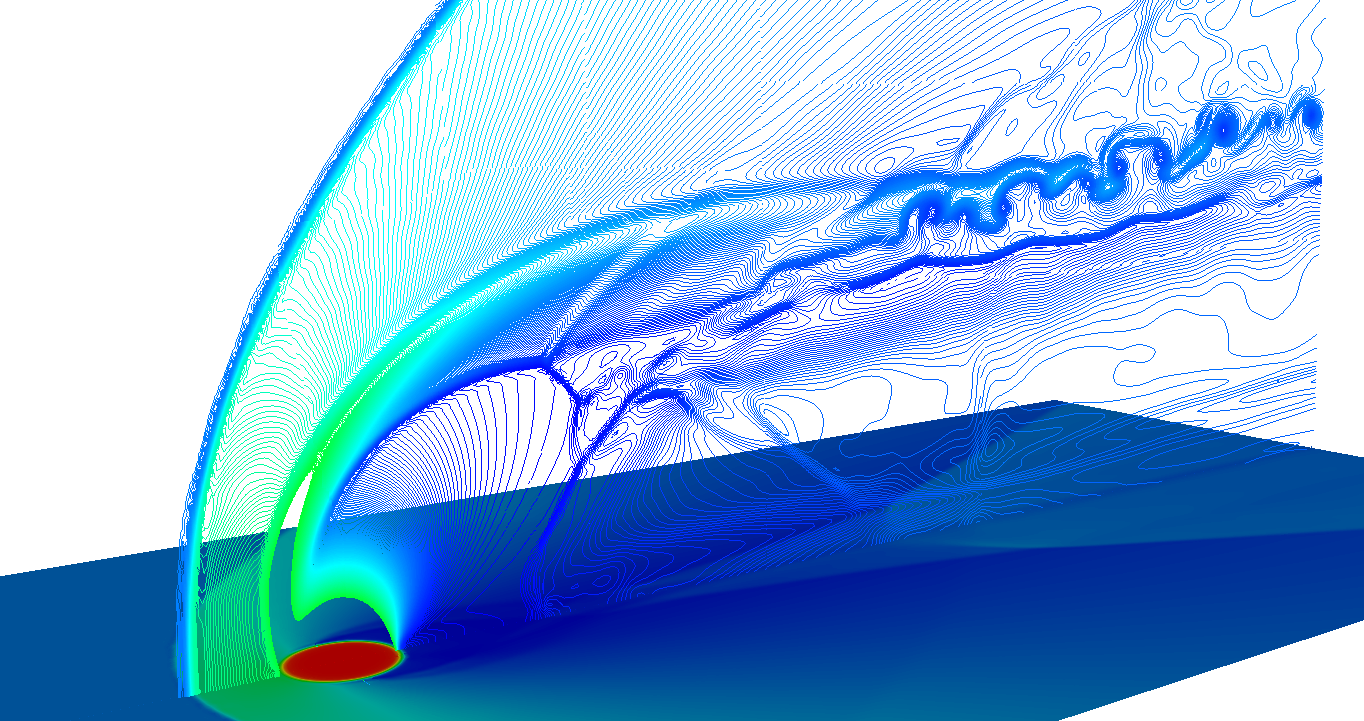
\includegraphics[width=0.9\textwidth]{pjcf_28_density.eps} \\
  \scriptsize Density
\end{center}
\end{frame}

\begin{frame}{
%
Runtime Benchmark
%
}
\begin{itemize}
  \item Benchmark with hybrid parallel computing.
  \begin{itemize}
    \item MPI across nodes; pthread within a node.
    \item Run on Glenn@OSC: 4 cores/node with 10Gbps IB.
  \end{itemize}
  \item Performance in million elements per second (Meps).
\end{itemize}
\begin{center} \footnotesize
  \begin{tabular}{ll|cccc}
  \multicolumn{2}{l|}{Number of cells (M)}
                            & 1     & 11   & 34   & 66   \\
  \hline
  Perf. (Meps) &    1 core  & 0.035 & --   & --   & --   \\
               &    4 cores & 0.13  & --   & --   & --   \\
               &   16 cores & 0.45  & 0.47 & --   & --   \\
               &   32 cores & --    & 0.91 & --   & --   \\
               &   44 cores & --    & 1.26 & 1.33 & --   \\
               &   80 cores & --    & --   & 2.16 & --   \\
               &  136 cores & --    & --   & 3.61 & 3.82 \\
               &  264 cores & --    & --   & --   & 7.17 \\
               &  512 cores & --    & --   & --   & 12.7 \\
               & 1024 cores & --    & --   & --   & 20.0
  \end{tabular}
\end{center}
\end{frame}

\begin{frame}{
%
Scaling
%
}
\begin{columns}[c]
\begin{column}{.5\textwidth}
\begin{center}
  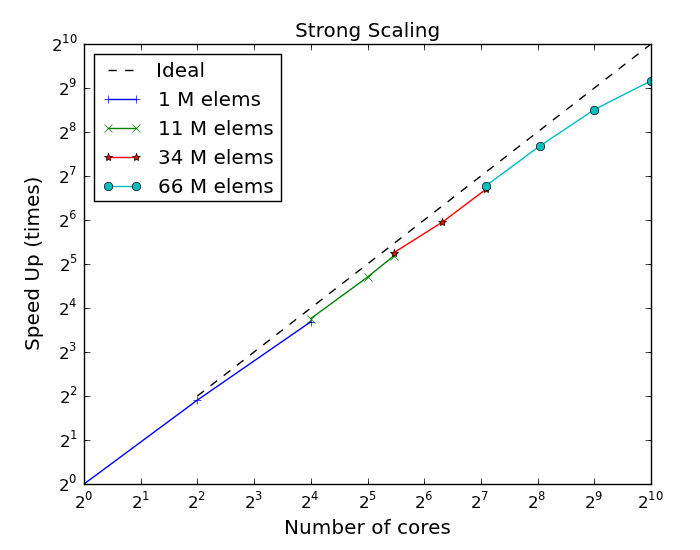
\includegraphics[width=\textwidth]{pjcf_speedup.eps} \\
  Fix Overall Mesh Size
\end{center}
\end{column}
\begin{column}{.5\textwidth}
\begin{center}
  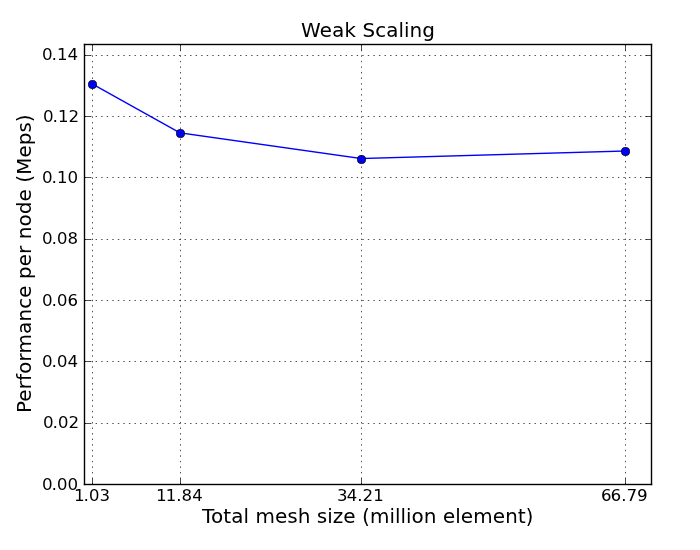
\includegraphics[width=\textwidth]{pjcf_weak.eps} \\
  Fix Per-Node Mesh Size
\end{center}
\end{column}
\end{columns}
\end{frame}

\subsection{
%%
Software System Structure
%%
}

\begin{frame}{
%
Two-Loop Structure of PDE Solvers
%
}
\begin{columns}[c]
\begin{column}{.5\textwidth}
\begin{itemize}
  \item The basic execution flow of SOLVCON:
  \begin{itemize}
    \item Temporal loop for temporal (or pseudo-temporal) integration.
    \item Spatial loops iterate over elements.
  \end{itemize}
  \item The structure is general to all PDE solvers.
\end{itemize}
\end{column}
\begin{column}{.5\textwidth}
  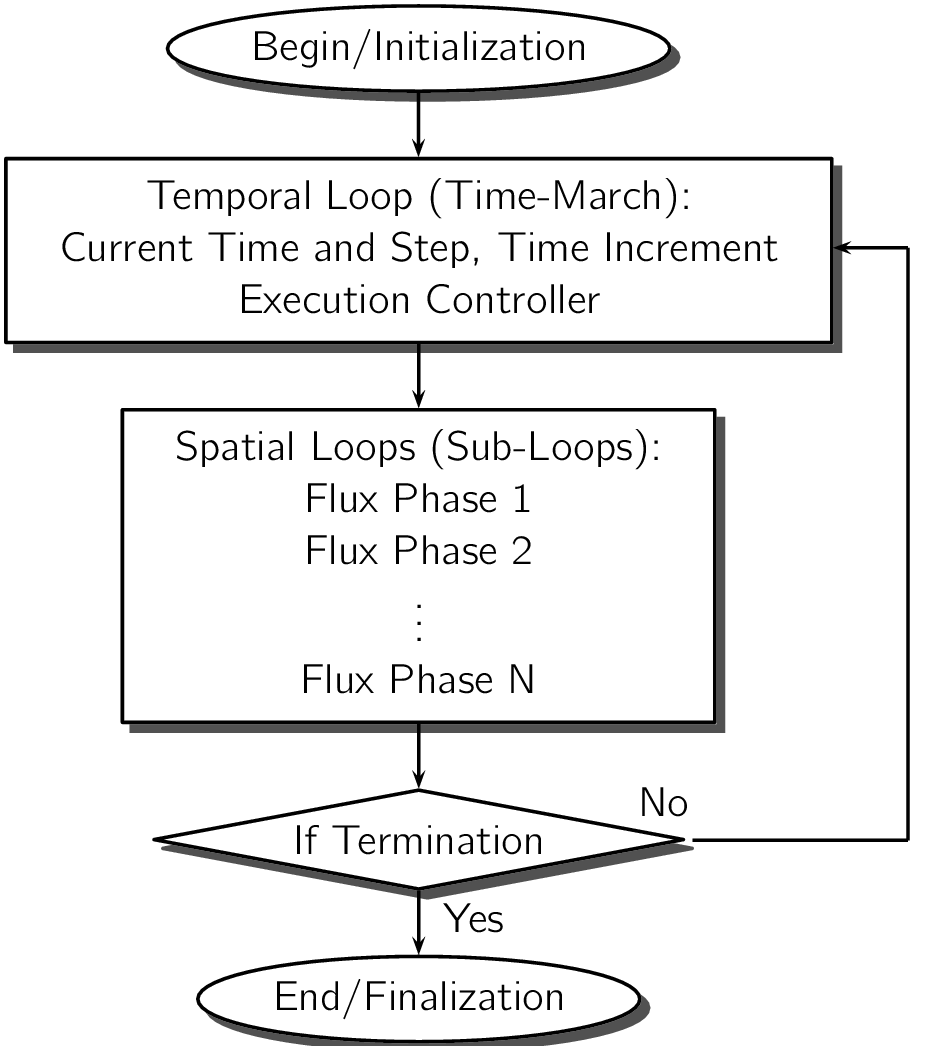
\includegraphics[width=.9\textwidth]{twoloop.eps}
\end{column}
\end{columns}
\end{frame}

\begin{frame}{
%
Solver Kernel for Spatial Loops
%
}
\begin{columns}[c]
\begin{column}{.75\textwidth}
\begin{itemize}
  \item A solver kernel is a Python class.
  \item The base class implements utility methods for \alert{spatial loops}.
  \item The algorithms directly work with the mesh look-up tables.
  \item The concrete solver implements real algorithms, in \alert{C}, or other
  fast languages.
\end{itemize}
\end{column}
\begin{column}{.25\textwidth} \centering
  \includegraphics[width=\textwidth]{inheritance.eps}
\end{column}
\end{columns}
\end{frame}

\begin{frame}{
%
Inheritance for Multi-Physics
%
}
\begin{itemize}
  \item For a multi-physics algorithm, like the CESE method, a class hierarchy
  can be designed to host multiple physical processes.
\end{itemize}
\begin{columns}[c]
\begin{column}{.5\textwidth}
\begin{itemize}
  \item The physical processes are segregated.
\end{itemize}
\end{column}
\begin{column}{.5\textwidth} \centering
  \includegraphics[width=\textwidth]{mphysics.eps}
\end{column}
\end{columns}
\end{frame}

\begin{frame}{
%
Temporal Loop and Call-Back
%
}
\begin{itemize}
  \item A standalone class hierarchy (\texttt{Case}) is designed to host the
  \alert{temporal loop}.
\end{itemize}
\begin{center}
  \parbox{\textwidth}{\centering
  \includegraphics[width=\textwidth]{lazy.eps}}
\end{center}
\begin{itemize}
  \item \texttt{Hook} and \texttt{Anchor} are call-back objects for
  \texttt{Case} and \texttt{Solver}, respectively.
  \begin{itemize}
    \item Supplement of main algorithms.
    \item Lazy initialization.
    \item Facilitating parallel computing and in-situ analysis.
  \end{itemize}
\end{itemize}
\end{frame}

\begin{frame}{
%
Overall Design of SOLVCON
%
}
\begin{center}
  \parbox{\textwidth}{\centering
  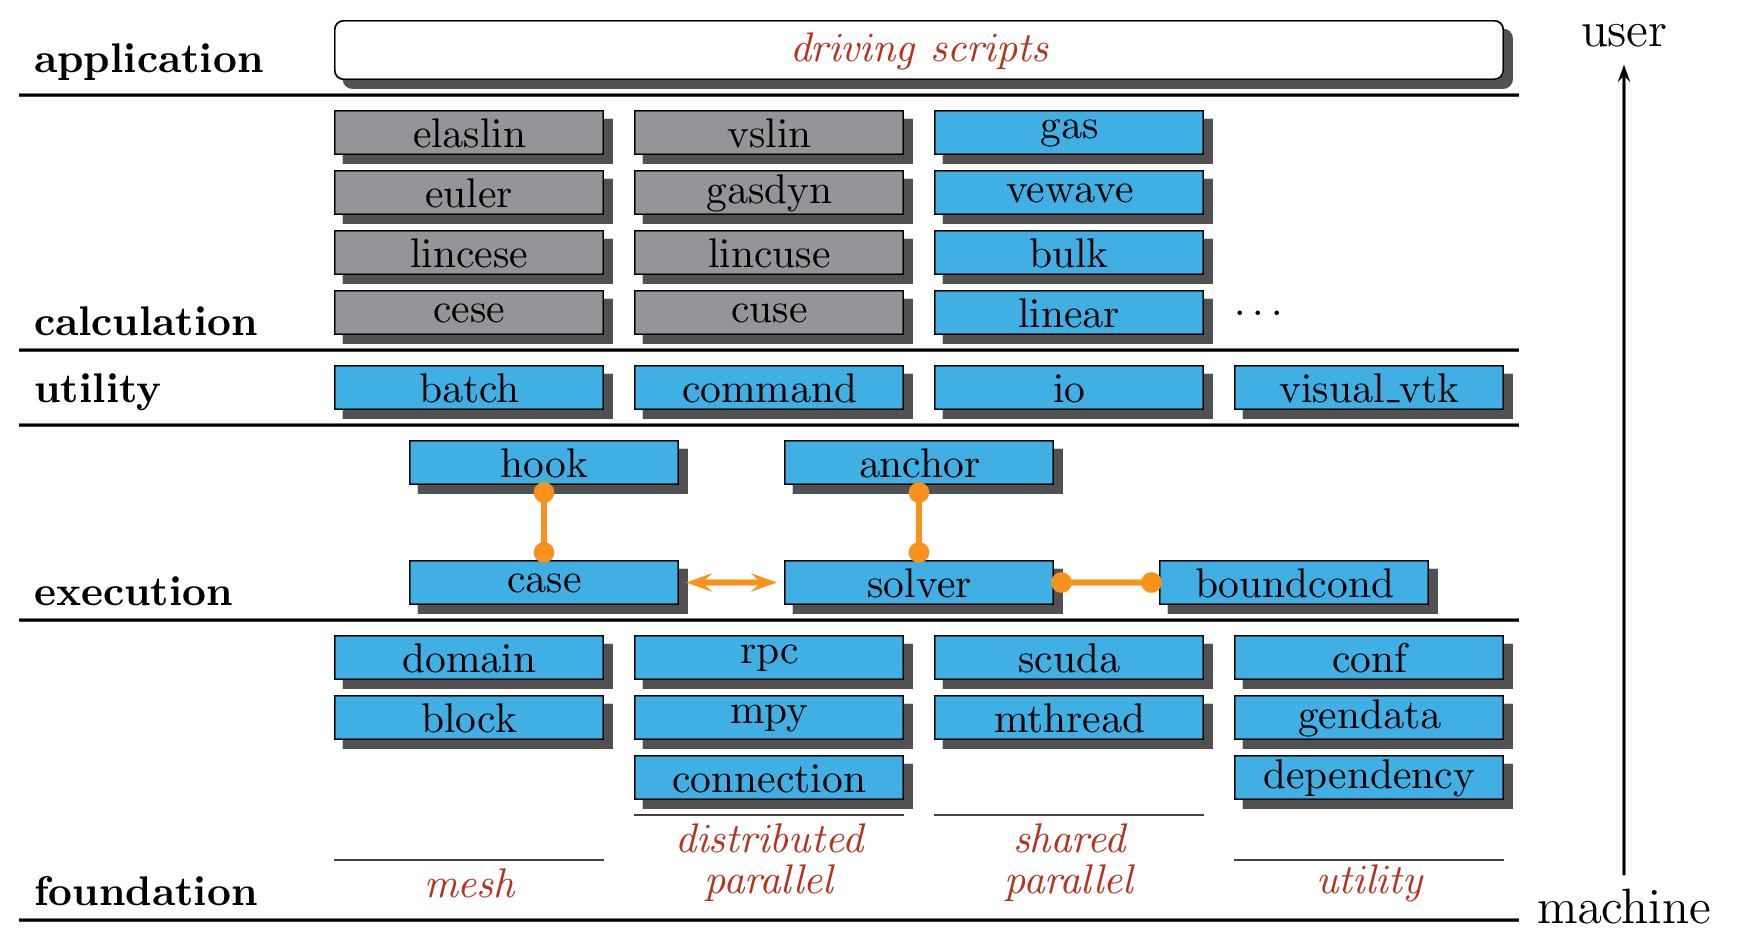
\includegraphics[width=\textwidth]{stack.eps}}
\end{center}
\end{frame}

\begin{frame}{
%
Renovation under Construction
%
}
\begin{center}
  \parbox{\textwidth}{\centering
  \includegraphics[width=0.9\textwidth]{stack_planned.eps}}
\end{center}
\begin{itemize} \footnotesize
  \item Simplify the architecture: Rely more on mpi4py, OpenMP, etc.
  \item Use Cython instead of ctypes for maintainability.
\end{itemize}
\end{frame}

\subsection{
%%
Parallel Computing
%%
}

\begin{frame}{
%
Two Types of Parallel Computing
%
}
\begin{minipage}[c]{\textwidth}\centering \footnotesize
\parbox{0.3\textwidth}{\centering 
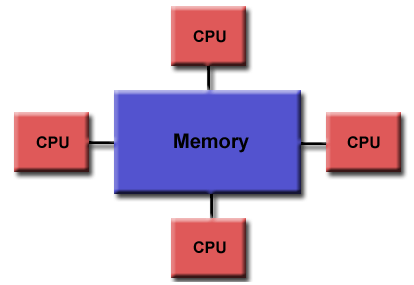
\includegraphics[width=0.3\textwidth]{mem_shared.eps} \\ \scriptsize shared
(multi-/many-core)}
+ 
\parbox{0.3\textwidth}{\centering
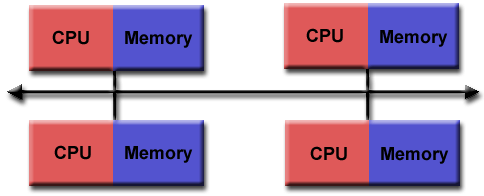
\includegraphics[width=0.3\textwidth]{mem_distributed.eps} \\ \footnotesize
distributed (cluster)}
= 
\parbox{0.3\textwidth}{\centering
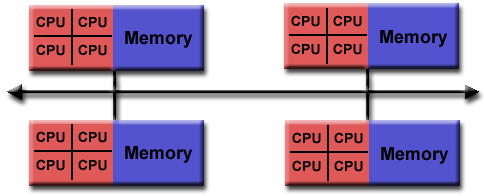
\includegraphics[width=0.3\textwidth]{mem_hybrid.eps} \\ \footnotesize hybrid}
\end{minipage}
\begin{itemize}
  \item Simultaneously use shared-memory and distributed-memory parallel
  computing (DMPC \& DMPC, respectively).
  \begin{itemize}
    \item Main difference: \alert{Addressing space}.
  \end{itemize}
  \item Inter-process communication is needed.
  \begin{itemize}
    \item DMPC is much more complex than SMPC.
    \item \alert{DMPC determines the scalability}.
    \item \alert{MapReduce is unsuitable}.
  \end{itemize}
\end{itemize}
\end{frame}

\begin{frame}{
%
Extending Solver Kernel for SMPC
%
}
\begin{columns}[c]
\begin{column}{.75\textwidth}
\begin{itemize}
  \item A \texttt{Solver} class can be extended to use shared-memory parallel
  computing.
  \item Only the spatial loops are modified.
  \item Can use pthread, OpenMP, CUDA, OpenCL, etc.
\end{itemize}
\end{column}
\begin{column}{.25\textwidth} \centering
  \includegraphics[width=\textwidth]{sharedmemory.eps}
\end{column}
\end{columns}
\end{frame}

\begin{frame}{
%
Domain Decomposition for DMPC
%
}
\begin{itemize}
  \item Before computation: Domain decomposition.
  \begin{itemize}
    \item Use connectivity data to build the graph of cells.
    \item Partition the graph by calling SCOTCH library.
    \item Use the partitioned graph to decompose mesh data.
  \end{itemize}
\end{itemize}
\begin{center} \scriptsize
  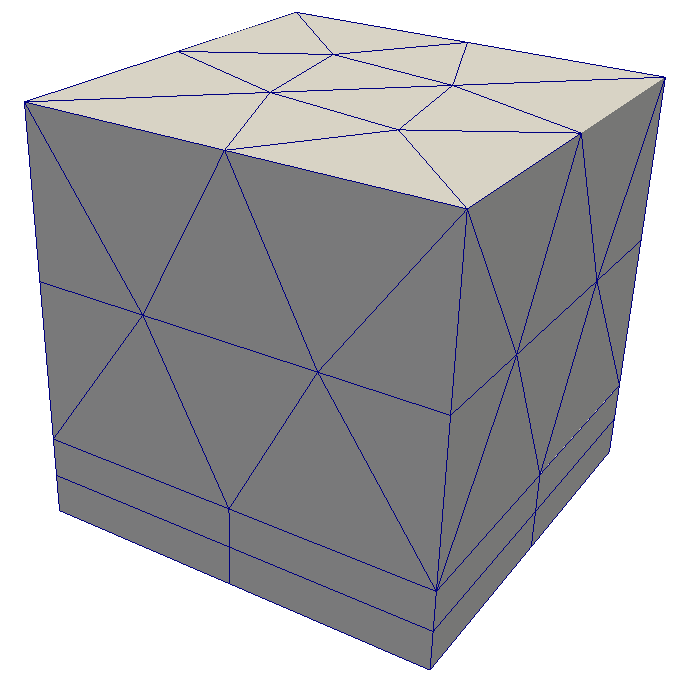
\includegraphics[width=0.2\textwidth]{mixed_mesh.eps}
  $\rightarrow$
  \includegraphics[width=0.25\textwidth]{meshgraph.eps}
  $\rightarrow$
  \includegraphics[width=0.25\textwidth]{meshgraph_partition.eps}
  $\rightarrow$
  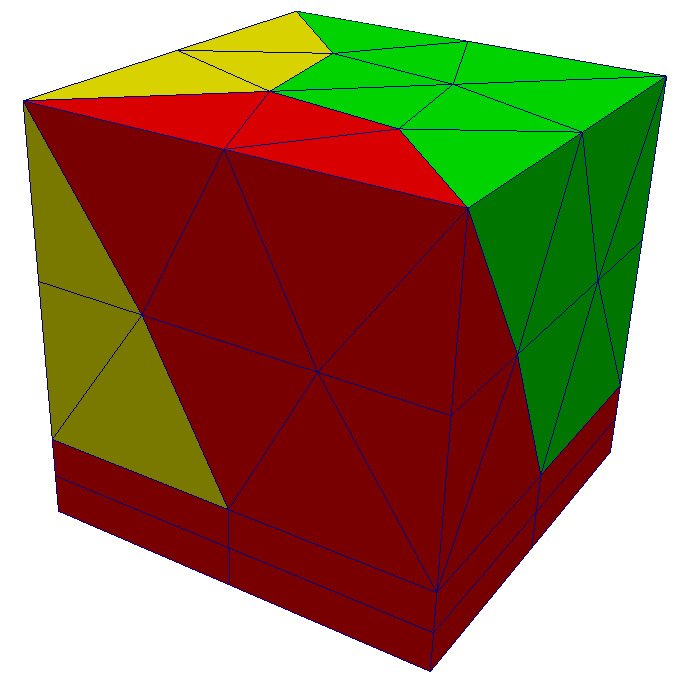
\includegraphics[width=0.2\textwidth]{mixed_mesh_decompose.eps}
\end{center}
\begin{itemize}
  \item During computation: Exchange data of the cells on the interface of
  different sub-domains.
  \begin{itemize}
    \item Use MPI to communicate among sub-domains.
  \end{itemize}
\end{itemize}
\end{frame}

\begin{frame}{
%
Solver Kernels Need Not Know DMPC
%
}
\begin{columns}[c]
\begin{column}{.3\textwidth}
\begin{itemize}
  \item DMPC is in SOLVCON framework.
  \item SMPC is in solver kernels.
\end{itemize}
\end{column}
\begin{column}{.7\textwidth} \centering \footnotesize
  DMPC Execution Flow in SOLVCON \\
  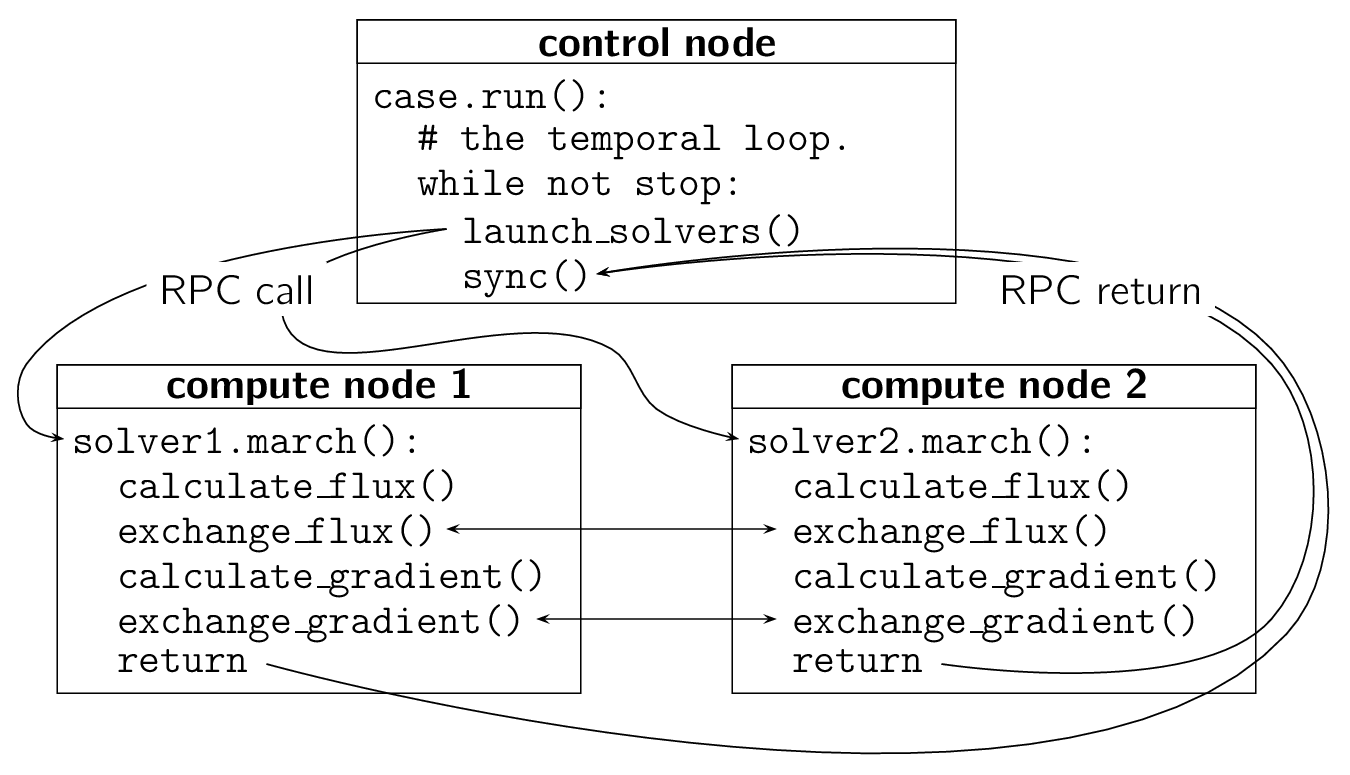
\includegraphics[width=\textwidth]{discomp.eps}
\end{column}
\end{columns}
\begin{itemize}
  \item When developing solver kernels, we do not need to worry about the
  complexity of DMPC.
  \item Hybrid parallelism is achieved by the segregation.
\end{itemize}
\end{frame}

\begin{frame}{
%
Post-Processing is Bottleneck
%
}
\begin{itemize}
  \item High-resolution simulations generate a lot of data:
  \begin{itemize}
    \item For 50 million element mesh, the data for one scalar
    (single-precision) are \alert{200 MB}.
    \item A typical run has at least 10,000 time steps.
    \item Transient analysis: $10,000 \times 200 \,\mbox{MB} = \alert{2
    \,\mbox{TB}}$.
    \item $\rho, p, T, \vec{v}, \vec{\omega}$ for CFD: $2 \,\mbox{TB} \times 9 =
    \alert{18 \,\mbox{TB}}$.
  \end{itemize}
  \item Workaround: Reducing output frequency.
  \begin{itemize}
    \item Every 100 time steps: \alert{180 GB}.
  \end{itemize}
  \item Post-processing the solutions is painfully time-consuming:
  \begin{itemize}
    \item The large data are usually processed by using a single workstation.
    \item Turnaround time could be in months.
  \end{itemize}
\end{itemize}
\end{frame}

\begin{frame}{
%
Solutions in SOLVCON
%
}
\begin{itemize}
  \item Parallel I/O.
  \begin{itemize}
    \item Each sub-domain outputs its own solutions.
    \item It is used with \alert{parallel post-processing}.
  \end{itemize}
  \item In situ visualization.
  \begin{itemize}
    \item Visualization is being done on the fly with the simulation.
    \item Everything happens in memory.
    \item Output only graphic files, which are much smaller than the full
    solution field.
  \end{itemize}
  \item Parallel I/O and in situ visualization are complementary to each other.
\end{itemize}
\end{frame}

\section*{
%%%
Conclusions
%%%
}

\begin{frame}{
%
Python: Rich Ecosystem for Scientists
%
}
\begin{itemize}
  \item Robust fundamental tools: NumPy, SciPy, Matplotlib, iPython, Cython.
  \item Abundant applications: Pandas, NLTK, networkx, VTK, PyMOL, Pyomo, ...,
  etc.
  \item iPython notebook is an excellent workbench from prototyping to
  presentation.
  \item Cython can help us to get the speed of C.
  \item A ``virtual lab'' can be built upon Python, like what SOLVCON is
  approaching.
\end{itemize}
\end{frame}

\begin{frame}{
%
Coding HPC for Research
%
}
\begin{itemize}
  \item Identifying the fundamental structure.
  \begin{itemize}
    \item In SOLVCON it's the two-loop structure.
    \item Enabled by the insights from the ``domain experts''.
  \end{itemize}
  \item Use Python from the beginning and to the end.
  \begin{itemize}
    \item Prototype your system with Python.
    \item Gradually replace performance hot spots with Cython or low-level C.
    \item Try to stay away from C++ or Fortran as much
    as possible.
  \end{itemize}
  \item It's very \alert{productive}.
  \begin{itemize} \normalsize
    \item SOLVCON is multi-physics by its clear structure with hybrid
    parallelism.
    \item Python rocks.
  \end{itemize}
\end{itemize}
\end{frame}

\begin{frame}{
%
%
}
\begin{center}
Thanks!
\end{center}
\end{frame}

\end{document}

% vim: set spell:
